% "{'classe':('PSI'),'chapitre':'chs_hs','type':('colle'),'titre':'Nacelle articulée grande portée', 'source':'XENS PSI 2019','comp':[],'corrige':True}"
%\setchapterimage{bandeau}
\chapter*{Colle \arabic{cptColle} \\ 
Nacelle articulée grande portée -- 
\ifprof Corrigé \else Sujet \fi}
\addcontentsline{toc}{section}{Colle \arabic{cptColle} :
Nacelle articulée grande portée -- 
\ifprof Corrigé \else Sujet \fi}

\iflivret \stepcounter{cptColle} \else
\ifprof  \stepcounter{cptColle} \else \fi
\fi

\setcounter{question}{0}
\marginnote{XENS PSI 2019.}
%\marginnote[1cm]{
%\UPSTIcompetence[2]{C1-02}
%\UPSTIcompetence[2]{C2-04}}

%\begin{marginfigure}[4cm]
%\centering
%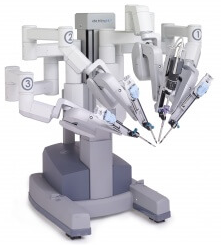
\includegraphics[width=4cm]{fig_00}
%\end{marginfigure}





%PSI XENS 2019
\ifprof
\else
\begin{marginfigure}
\centering
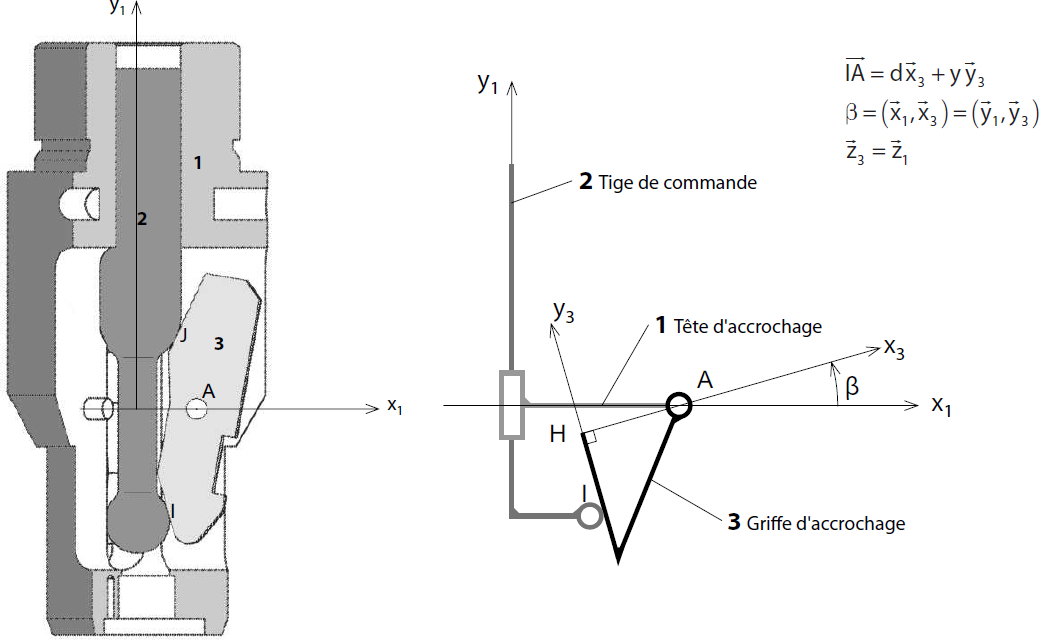
\includegraphics[width=\linewidth]{fig_01}
\caption{Architecture globale de la nacelle \label{fig_01}}
\end{marginfigure}

La nacelle articulée (Figure \ref{fig_01}) étudiée permet de sécuriser des opérations de travail en hauteur. 
Cette nacelle s’utilise en extérieur et est adaptée à tous les terrains grâce à ses 4 roues motrices 
et son essieu oscillant. Elle est principalement utilisée pour : la construction de gros et second 
œuvre, l’aménagement d’espaces verts, la logistique, la distribution et l’industrie, la maintenance 
et la restauration. 


La nacelle est amenée à évoluer dans des terrains parfois accidentés (chantier, terrain en friche…).
L’objectif est de valider la motricité du châssis par rapport au sol, même sur un terrain accidenté. 
Le châssis possède un essieu avant monté sur un palonnier pilotable par deux vérins. 

\begin{marginfigure}
\centering
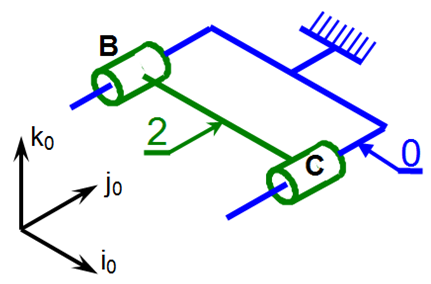
\includegraphics[width=\linewidth]{fig_02}
\caption{Modèle du châssis \label{fig_02}}
\end{marginfigure}


$C_1$, $C_1'$, $C_2$, $C_2'$ sont les centres respectivement des roues avant droite, avant gauche, arrière droite 
et arrière gauche. Les quatre roues sont considérées en liaison ponctuelle parfaite avec le sol. Les 
points de contact sont notés respectivement $F_1$, $F_1'$, $F_2$, $F_2'$. 
\fi


%\question{Réaliser le graphe de liaisons.}
%\ifprof
%\begin{corrige}~\\
%\begin{center}
%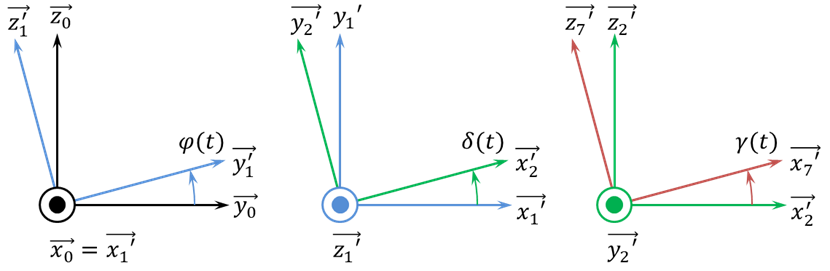
\includegraphics[width=.5\linewidth]{cor_01}
%\end{center}
%\end{corrige}
%\else\fi

\question{Tracer le graphe de structure.}

\question{Déterminer le degré d’hyperstatisme du modèle de la figure \ref{fig_02} sans les vérins et 
indiquer si ce modèle permet ou non de conserver le contact avec chacune des roues quelle que 
soit la forme du terrain.}
\ifprof
\begin{corrige}
\textbf{Méthode cinématique : $h = m - I_c + E_c$}
\begin{itemize}
\item $m=7$ : 4 rotations indépendantes des 4 roues autout des axes $\axe{C}{y_0}$, le véhicule sur un plan a 3 mobilités (translations suivant $\vx{0}$ et $\vy{0}$) rotation autour de $\vz{0}$;
\item 5 pivots avec une inconnue cinématique chacune et 4 contacts ponctuels (5 inconnues cinématiques) $I_c = 5\times 1 + 4\times 5 = 25$;
\item 7 solides, 9 liaisons soient $\gamma = 9-7+1 = 3$ et $E_c = 6\times 3 = 18$.
\end{itemize}
Au final : $h = m - I_c + E_c= 7 - 25 + 18 = 0$.
\end{corrige}
\else\fi

\textbf{Les vérins ne sont toujours pas pris en compte.}

\question{Etablir la liaison équivalente réalisée par l'essieu avant entre le sol et le châssis. 
Donner chaque étape de la démarche.}
\ifprof
\begin{corrige}
La liaison ponctuelle de normale $\axe{F_1}{z_0}$ et la pivot d'axe $\axe{C_1}{y_0}$ sont en parallèle. Pour déterminer le torseur équivalent on somme les torseurs cinématiques :
$\torseurcin{V}{\text{Es}}{\text{RAv}} + \torseurcin{V}{\text{RAv}}{\text{Sol}}$
$=\torseurl{\alphap \vy{0}}{\vect{0}}{C_1}+\torseurl{\betap_x \vx{0}+\betap_y \vy{0}+\betap_z \vz{0}}{\lambdap_x\vx{0}+\lambdap_y\vy{0}}{C_1}$
$=
\torseurl{\betap_x \vx{0}+\left(\alphap + \betap_y \right)\vy{0}+\betap_z \vz{0}}{\lambdap_x\vx{0}+\lambdap_y\vy{0}}{C_1}$.

Il s'agit donc d'une liaison ponctuelle de normale $\axe{C_1}{z_0}$.

\vspace{.4cm}

On est maintenant en présence de deux liaisons ponctuelle de normale $\axe{C_1}{z_0}$ et $\axe{C'_1}{z_0}$. La liaison équivalente est une liaison linéaire rectiligne (cylindre -- plan) de normale 
$\axe{H_1}{z_0}$ et de direction $(C_1C'_1)$.

\vspace{.4cm}

Enfin, la liaison linéaire rectiligne et la liaison pivot sont en série. Pour déterminer le torseur équivalent on somme les torseurs cinématiques :
$\torseurcin{V}{\text{Ch}}{\text{Ess}} + \torseurcin{V}{\text{Ess}}{\text{Sol}}$
$=\torseurl{\gammap \vy{0}}{\vect{0}}{H_1}+\torseurl{\deltap_y \vy{0}+\deltap_z \vz{0}}{\mup_x\vx{0}+\mup_y\vy{0}}{H_1}$

$=\torseurl{\left(\gammap +\deltap_y \right)\vy{0}+\deltap_z \vz{0}}{\mup_x\vx{0}+\mup_y\vy{0}}{C_1}$.

La liaison équivalente est une liaison linéaire rectiligne (cylindre -- plan) de normale 
$\axe{H_1}{z_0}$ et de direction $(C_1C'_1)$.

\begin{center}
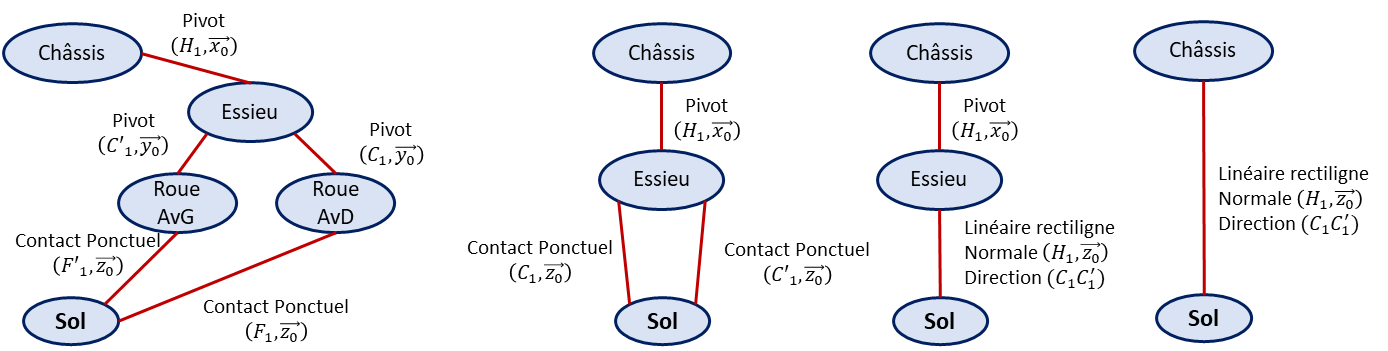
\includegraphics[width=.8\linewidth]{cor_02}
\end{center}

\end{corrige}
\else\fi

\question{Donner l’avantage de la solution constructeur par rapport à une solution à 4 roues 
directement sur le châssis et par rapport à une solution à 3 roues directement sur le châssis.}
\ifprof
\begin{corrige}
Cette solution permet d'avoir toujours les 4 roues en contact avec le sol, quelque soit le terrain, même s'il est accidenté. 
\end{corrige}
\else\fi

\question{Donner le rôle des vérins et indiquer selon quels critères ils peuvent être pilotés.}
\ifprof
\begin{corrige}
Le mécanisme est isostatique. Le maintien du contact entre les roues et le sol sera garanti par un pilotage adéquat des vérins.
\end{corrige}
\else\fi


\textbf{Les vérins sont maintenant pris en compte.}

\question{En utilisant le modèle de la figure \ref{fig_02}, proposer une liaison entre le corps du vérin d'une part et le châssis d'autre part. Proposer ensuite une liaison entre la tige du vérin d'une part et l'essieu avant d'autre part. Tracer un schéma cinématique de le solution proposée.}
\ifprof
\begin{corrige}
Le vérin peut être lié de part et d'autre par une liaison rotule de part et d'autre. 
\end{corrige}
\else\fi

\ifprof
\else
\begin{marginfigure}
\centering

\includegraphics[width=3cm]{Cy_06_02_Colle_04_Nacelle_qr}
\end{marginfigure}
\fi


\question{Tracer le nouveau graphe de structure puis déterminer le degré d'hypestatisme du mécanisme.}
\ifprof
\begin{corrige}
On ajoute 2 liaisons rotules par vérin et une liaison pivot glissant par vérin.
On a donc : 
\begin{itemize}
\item $m=7+2+2 = 11$ : un ensemble vérin peut pivoter sur son axe et la tige peut aussi pivoter sur son axe ;
\item on ajoute 4 rotules et 2 pivot glissant ; $I_c = 5\times 1 + 4\times 5+ 4\times 3+ 2\times 2 = 25+12+4 = 41 $;
\item on ajoute 4 solides et 6 liaisons soient $\gamma = 9+6-7-4+1 = 5$ et $E_c = 6\times 5 = 30$.
\end{itemize}
On a donc $h=m-I_c+E_c = 11 - 41 + 30 =0$. Le mécanisme reste isostatique avec les vérins. 
\end{corrige}
\else\fi
